
\begin{figure*}
\begin{center}
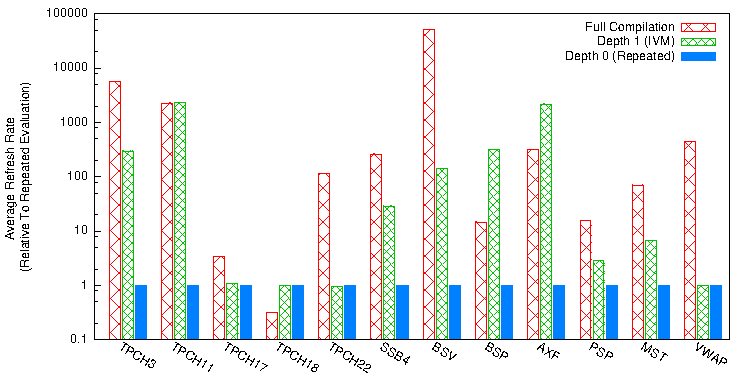
\includegraphics[width=\textwidth]{../graphs/graphs/bakeoff.pdf}
\caption{Cross-query comparison of our compiler in different depth-restricted modes, and the best performing streaming and database engine for each query.  Note the logscale on the y-axis.}
\label{fig:experiments:bakeoff}
\end{center}
\end{figure*}

We now analyze the performance of \dbtoaster.  As in Section \ref{sec:dbfail}, experiments are run on \todo{insert hardware configuration here}. 
 
Our analysis uses the queries from Examples \ref{ex:dbfail:stock}(PRICESPREAD),  \ref{ex:dbfail:tpch}(SHIPPING), and \ref{ex:dbfail:network}(SERVERLOAD), Queries numbers 3, 11, 17, 18, and 22 from the TPC-H\cite{tpch} benchmark, the VWAP query presented in \cite{kennedy-ahmad-koch-cidr:11}, and four additional financial queries: MISSEDTRADES, AXFINDER, BROKERSPREAD, and BROKERCOVARIANCE in the spirit of VWAP and PRICESPREAD.  These queries are presented in \todo{reference these queries somehow?}.

Queries were run on pre-generated traces until completion of the trace or a 1 hour cutoff.  Trace files are processed as follows: The financial queries: VWAP, MISSEDTRADES, AXFINDER, BROKERSPREAD, PRICESPREAD, and BROKERVARIANCE were run on a 2 million tuple trace of stock market activity for MSFT.  The TPCH-H and SHIPPING queries were run on a database generated by dbgen\cite{tpch} with scaling factor 0.1 (100 MB).  Insertions are drawn from the data files for each table and interleaved in random order \todo{weighted by the final size of each table}.  The SERVERLOAD query was run on a synthetically generated dataset using 1000 racks of 20 servers each, and 100,000 status updates each instantiated as a deletion followed by an insertion.

For comparison, we use a depth-limited instantiation of our compilation algorithm where maps are not materialized beyond a fixed number of recursive steps.  Compilation limited to depth 1 is approximately equivalent to traditional IVM techniques, while depth 0 is equivalent to re-evaluating the query on every insertion\footnote{We have implemented an in-memory query processing engine to support depth 1 and depth 0 compilation.  Although the capabilities of this engine are limited, we do not expect further optimizations  to have a meaningful impact on the processing times of our test queries.}

Note that \dbtoaster\ is able to take advantage of the TPC-H benchmark's append-only nature: The SHIPPING and the TPC-H queries are compiled without deletion triggers.  As a further optimization, all queries involving strings use a dictionary to compress string data before processing.

\subsection{Equijoins}
\begin{figure*}
\begin{center}
\begin{tabular}{ccc}
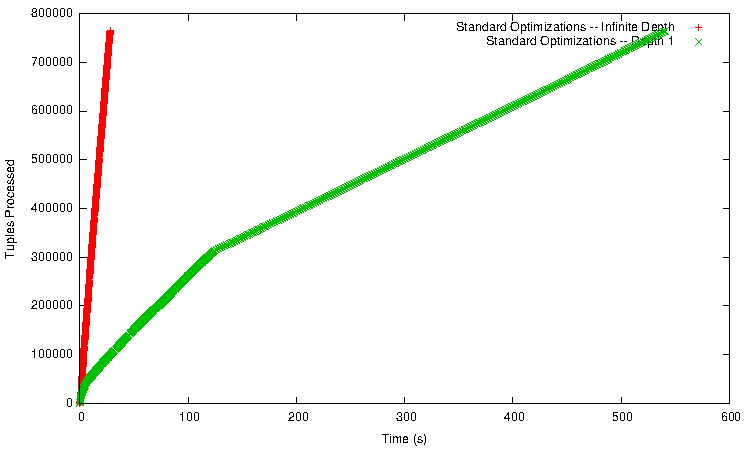
\includegraphics[width=2.2in]{../graphs/graphs/time_tpch3.pdf} &
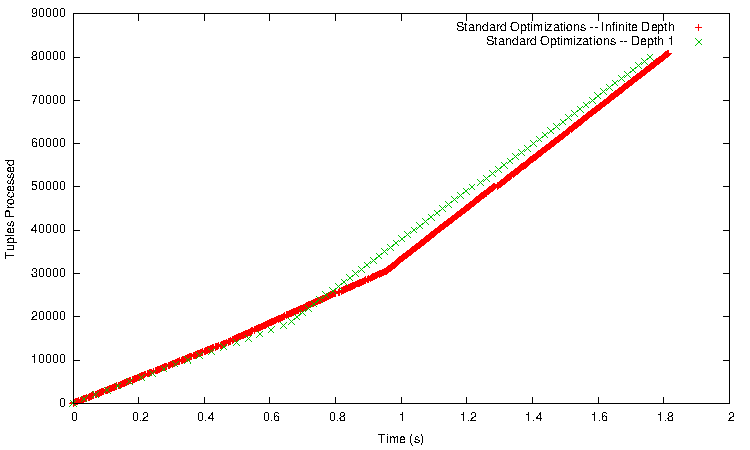
\includegraphics[width=2.2in]{../graphs/graphs/time_tpch11.pdf} &
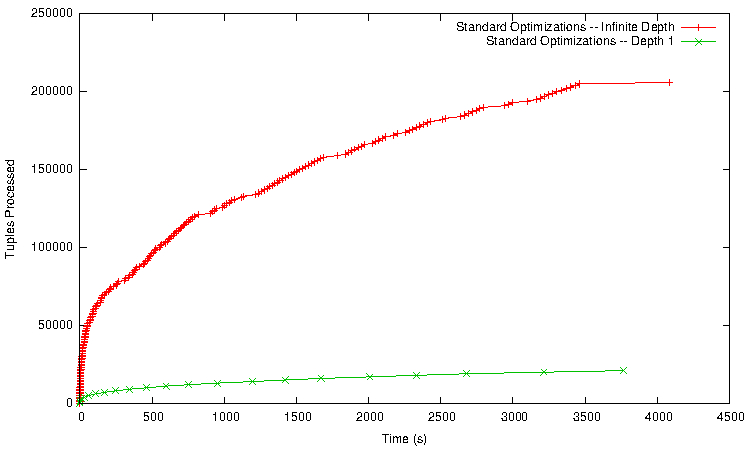
\includegraphics[width=2.2in]{../graphs/graphs/time_ssb4.pdf} \\
(a) & (b) & (c) \\
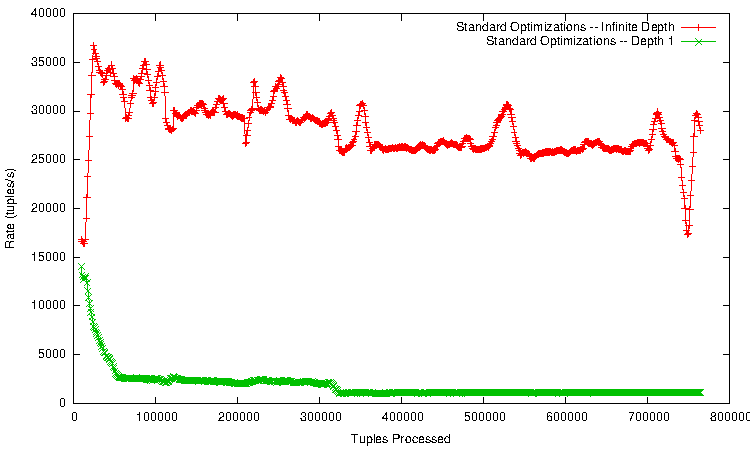
\includegraphics[width=2.2in]{../graphs/graphs/windowedrate_tpch3.pdf} &
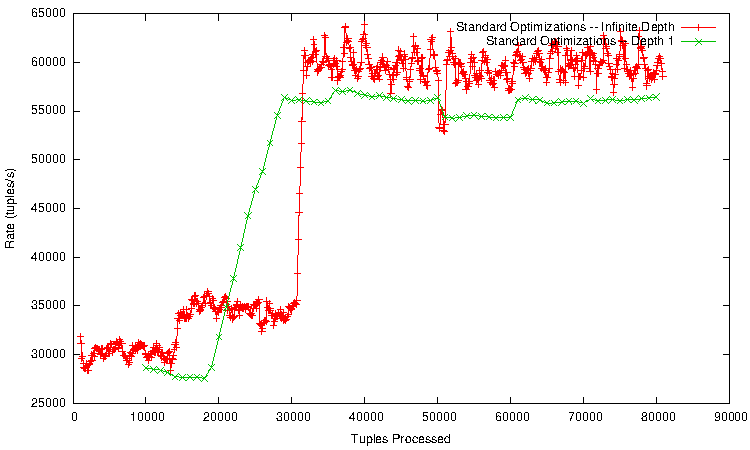
\includegraphics[width=2.2in]{../graphs/graphs/windowedrate_tpch11.pdf} &
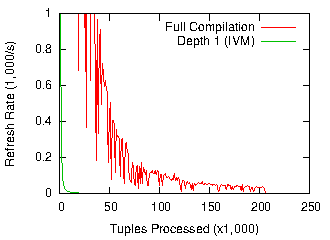
\includegraphics[width=2.2in]{../graphs/graphs/windowedrate_ssb4.pdf} \\
(d) & (e) & (f) \\
\end{tabular}
\caption{Cumulative number of tuples processed vs time (a-c) and tuple processing rate as a function of number of tuples inserted (d-f) on three equijoin queries: TPCH Query 11 (a,d), TPCH Query 2 (b,e), and SHIPPING (c,f)}
\label{fig:experiments:equijoin}
\end{center}
\end{figure*}

Figure \ref{fig:experiments:equijoin} shows the performance of our compiler on three equijoin queries.  TPCH Query 3 is a 3-way select-project-join-aggregate.  \todo{once we get the re-weighting right, the IVM curve should get a bit rounder.  Rewrite once this happens}.  TPCH Query 11 is the simplest query of the three, a 2-way equi-join on a one-to-many relationship (SUPPLIER to PARTSUPP) with bounded fanout.  SHIPPING is a 7-table star-join with a join-width of 6.  

Our compiler recurses only once on TPCH Query 11.  As a consequence, the result is nearly equivalent to IVM\footnote{We pre-aggregate the materializations of SUPPLIER and PARTSUPP, but this is only a minor improvement in practice due to the bounded fanout of this query}.  Both TPCH Query 3 and SHIPPING demonstrate a substantial performance increase over IVM.  The one-to-one, and bounded fanout one-to-many relationships between elements of many of these queries are actually advantageous to the IVM implementation -- each insertion only triggers a limited number of reads.  In spite of this, incrementally maintaining the (aggregate) delta queries results in a net reduction in the amount of work required -- especially in a large query like SSB4.

\todo{Do these results provide any concrete evidence of time complexity improvements?  not really... the foreign-key relationships reduce the IVM implementation's complexity in the same way... lets's see how serverload does... }

\subsection{Nested Subqueries}
\begin{figure*}
\begin{center}
\begin{tabular}{ccc}
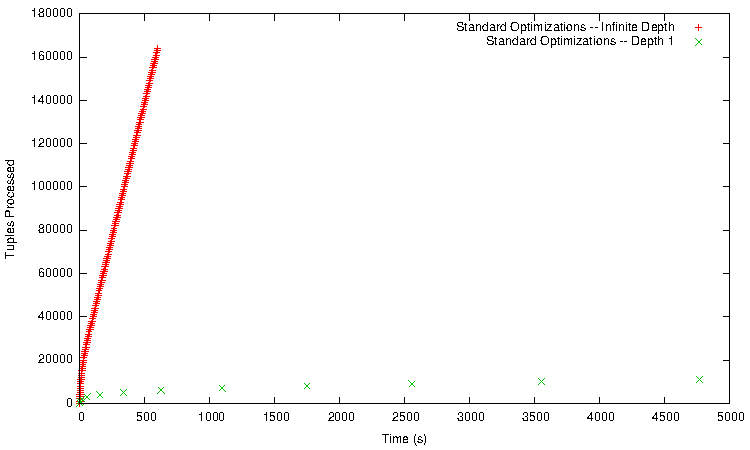
\includegraphics[width=2.2in]{../graphs/graphs/time_tpch22.pdf} &
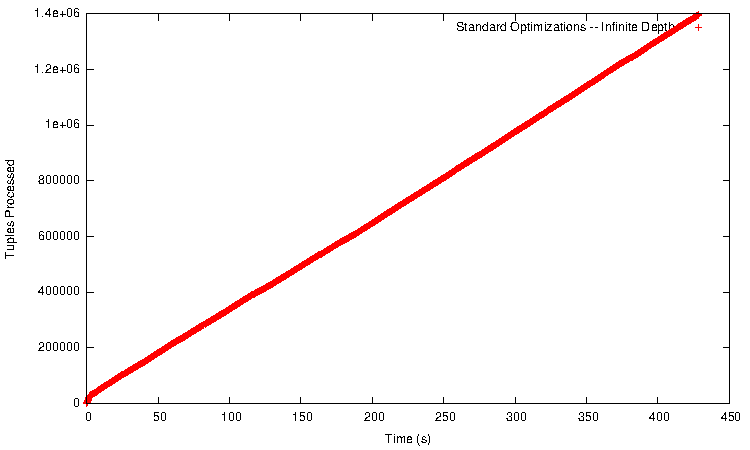
\includegraphics[width=2.2in]{../graphs/graphs/time_vwap.pdf} &
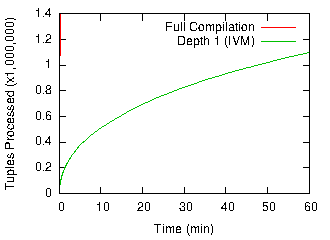
\includegraphics[width=2.2in]{../graphs/graphs/time_brokervariance.pdf} \\
(a) & (b) & (c) \\
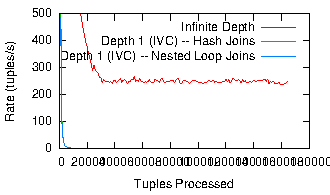
\includegraphics[width=2.2in]{../graphs/graphs/windowedrate_tpch22.pdf} &
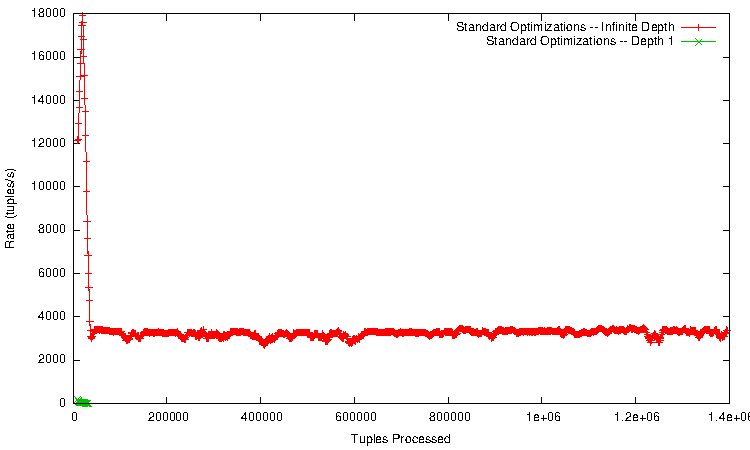
\includegraphics[width=2.2in]{../graphs/graphs/windowedrate_vwap.pdf} &
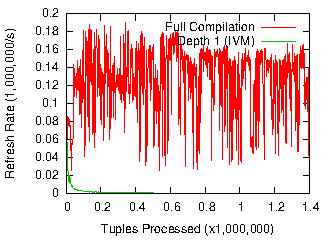
\includegraphics[width=2.2in]{../graphs/graphs/windowedrate_brokervariance.pdf} \\
(d) & (e) & (f) \\
\end{tabular}
\caption{Cumulative number of tuples processed vs time (a-c) and tuple processing rate as a function of number of tuples inserted (d-f) on three queriest: TPCH Query 22 (a,d), VWAP (b,e), and BROKERVARIANCE (c,f)}
\label{fig:experiments:nestedgood}
\end{center}
\end{figure*}


\begin{figure*}
\begin{center}
\begin{tabular}{ccc}
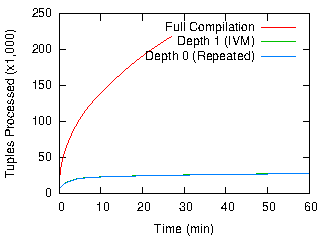
\includegraphics[width=2.2in]{../graphs/graphs/time_serverload.pdf} &
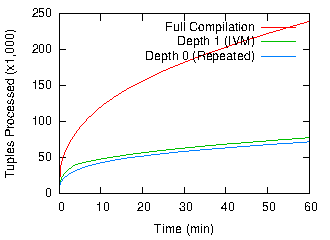
\includegraphics[width=2.2in]{../graphs/graphs/time_tpch17.pdf} &
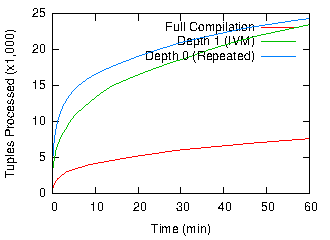
\includegraphics[width=2.2in]{../graphs/graphs/time_tpch18.pdf} \\
(a) & (b) & (c) \\
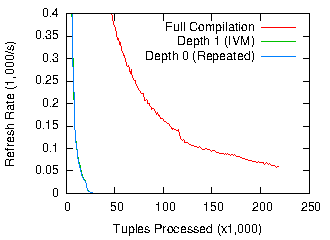
\includegraphics[width=2.2in]{../graphs/graphs/windowedrate_serverload.pdf} &
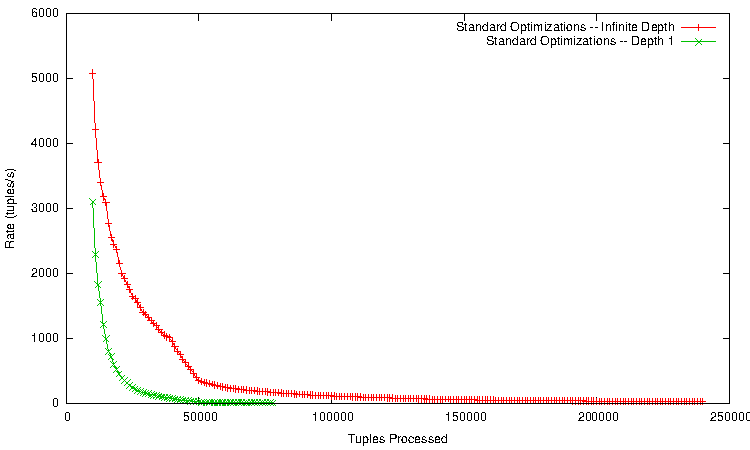
\includegraphics[width=2.2in]{../graphs/graphs/windowedrate_tpch17.pdf} &
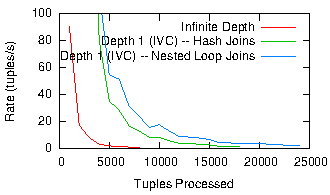
\includegraphics[width=2.2in]{../graphs/graphs/windowedrate_tpch18.pdf} \\
(d) & (e) & (f) \\
\end{tabular}
\caption{Cumulative number of tuples processed vs time (a-c) and tuple processing rate as a function of number of tuples inserted (d-f) on two queries with nested aggregates: SERVERLOAD (a,d), TPCH Query 17 (b,e), and TPCH Query 18}
\label{fig:experiments:nestedmeh}
\end{center}
\end{figure*}

Figures \ref{fig:experiments:nestedgood} and \ref{fig:experiments:nestedmeh} illustrate the performance of our compiler on several queries with nested aggregates.  

Of these, TPCH Query 22: queries with selection conditions based on a nested aggregate query\footnote{TPCH Query 22 also has a nested lookup, which is constant-time in both IVM and full compilation.}.  In IVM, the nested aggregate is recomputed on every update -- updates are linear in the number of tuples.  The nested aggregate contains no terms bound on the outside, so under full compilation the nested aggregate is incrementally maintained -- updates are effectively reduced to constant time.  

VWAP has a selection condition based on two nested aggregate queries.  One of the nested aggregates has an inequality condition over a variable not bound inside the expression.  As in TPCH Query 22, these aggregates are recomputed on every update.  The nested aggregate with an inequality condition over an externally bound variable is of interest.  Because the domain of the externally bound variable is determined outside of the nested aggregate, the fully compiled query must still re-evaluate the nested query every time it encounters a bid with a price that it has not seen before.  However, the domain of prices is bounded, so after an initial ramp up process (that occurs while the size of the table is small) the fully compiled query can incrementally maintain the query output.

Although it does not contain a nested aggregate, the performance of BROKERSPREAD follows a pattern similar to the prior two queries.  This is not surprising -- materializing the first order delta has the same effect as materializing the correlated aggregate into an incrementally maintained lookup table.  Furthermore, unlike TPCH Query 11 (Figure \ref{fig:experiments:equijoin}a,c), the join relationship is many-to-many and the number of matches grows over time.  Consequently, IVM must do more work with each iteration, while the fully compiled query's work remains constant.

%SERVERLOAD is bad because we never do domain cleanup.
SERVERLOAD is a query with a comparison over a nested aggregate, and should perform as well as the prior two queries.  The observed non-linear performance is a consequence of a limitation in our runtime implementation that prevents it from properly garbage collecting deleted entries in one of the generated lookup tables.  
\todo{Need a good way to spin the last paragraph...  someone paying attention might catch that the same issue that we have at infinite depth here is going to have a disproportionately negative impact on our depth 1 evaluation for not only this query but several of the finance ones too.}

TPCH Query 17 contains both a nested aggregate and a two-way join.  As in the prior two queries, incrementally maintaining the nested aggregate makes insertions into the LINEITEM table constant-time rather than linear.  However, even in the fully compiled query, insertions into the PART table must still iterate over all matching LINEITEM entries to compute the update to the query result.  In practice full compilation would perform even better, as the TPCH specification defines the join key as a foreign key dependency from LINEITEM to PART, while the random ordering of insertions in our tests results in some LINEITEMs being inserted before their corresponding PART.

\todo{Write up Query 18 after we get the revised numbers}

\subsection{Memory Limitations}
\begin{figure}
\begin{center}
\hspace*{-0.2in}
\begin{tabular}{cc}
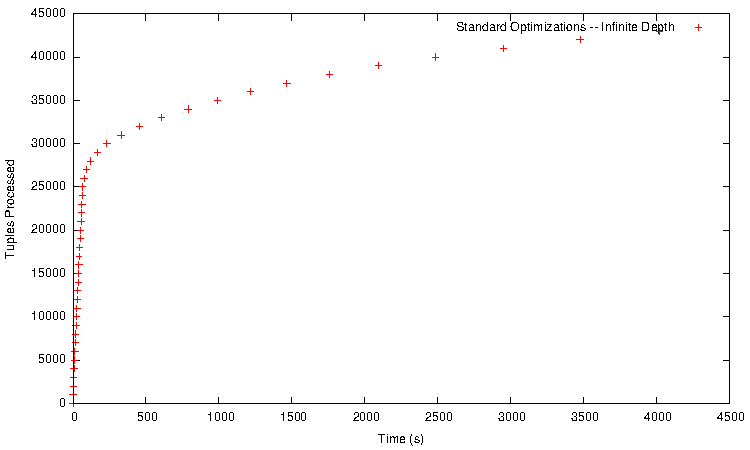
\includegraphics[width=1.7in]{../graphs/graphs/time_pricespread.pdf} &
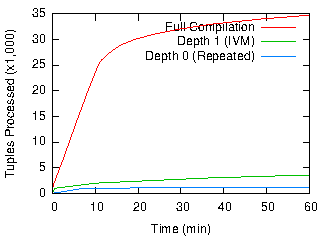
\includegraphics[width=1.7in]{../graphs/graphs/time_missedtrades.pdf} \\
(a) & (b) \\
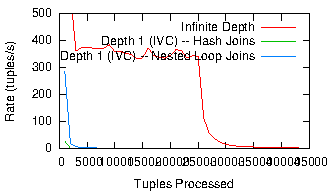
\includegraphics[width=1.7in]{../graphs/graphs/windowedrate_pricespread.pdf} &
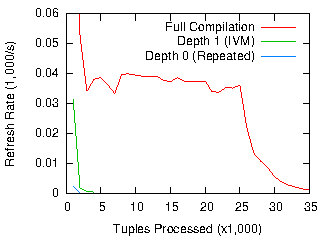
\includegraphics[width=1.7in]{../graphs/graphs/windowedrate_missedtrades.pdf} \\
(c) & (d) \\
\end{tabular}
\caption{Cumulative number of tuples processed vs time (a,b) and tuple processing rate as a function of number of tuples inserted (c,d) on two queries where memory becomes an issue: PRICESPREAD (a,c), MISSEDTRADES (b,d)}
\label{fig:experiments:memissues}
\end{center}
\end{figure}



\subsection{Map Extraction} 
\begin{figure}
\begin{center}
\hspace*{-0.2in}
\begin{tabular}{cccc}
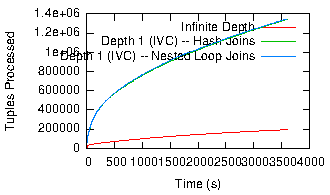
\includegraphics[width=1.7in]{../graphs/graphs/time_axfinder.pdf} &
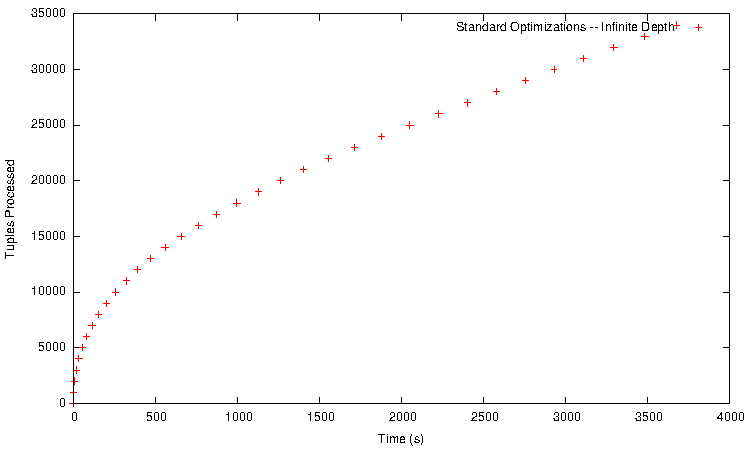
\includegraphics[width=1.7in]{../graphs/graphs/time_brokerspread.pdf} \\
(a) & (b) \\
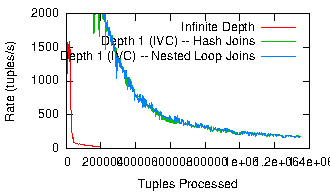
\includegraphics[width=1.7in]{../graphs/graphs/windowedrate_axfinder.pdf} &
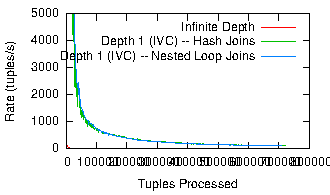
\includegraphics[width=1.7in]{../graphs/graphs/windowedrate_brokerspread.pdf} \\
(c) & (d) \\
\end{tabular}
\caption{Cumulative number of tuples processed vs time (a,b) and tuple processing rate as a function of number of tuples inserted (c,d) on two queries where our extraction heuristic chooses incorrectly: AXFINDER (a,c) and BROKERSPREAD (c,d)}
\label{fig:experiments:extraction}
\end{center}
\end{figure}

\subsection{Varying Depths}
\begin{figure}
\begin{center}
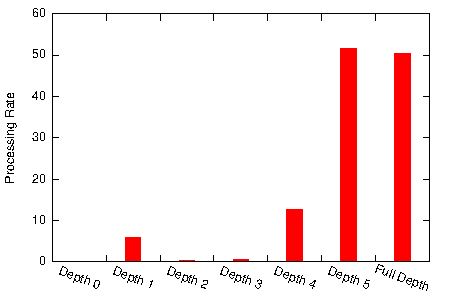
\includegraphics[width=3in]{../graphs/graphs/depth_ssb4.pdf}
\caption{Average processing rate as a function of compilation depth on SHIPPING.}
\label{fig:experiments:ssb4depth}
\end{center}
\end{figure}


\begin{figure}
\begin{center}
\begin{tabular}{|l|c|c|c|}\hline 
\ & Infinite Depth & Depth 1 & Depth 0 \\\hline 
TPCH3 & 2509 & 2855 & 4198 \\\hline
TPCH11 & 531 & 596 & 616 \\\hline
TPCH17 & 928 & 1158 & 1478 \\\hline
TPCH18 & 3668 & 3538 & 4631 \\\hline
TPCH22 & 777 & 1135 & 754 \\\hline
SSB4 & 10995 & 8954 & 7904 \\\hline
BSV & 342 & 327 & 347 \\\hline
BSP & 45625 & 567 & 729 \\\hline
AXF & 2169 & 553 & 1394 \\\hline
PSP & 1442 & 1878 & 1890 \\\hline
MST & 5457 & 2870 & 2434 \\\hline
VWAP & 533 & 466 & 341 \\\hline
\end{tabular}
\end{center}
\end{figure}